\chapter{Computer Arithmetic and Computational Errors}

\section{Numerical Stability}

There is only finite space in computer. How would we store \( \pi \), an irrational number? We can't. We can only store an approximation of \( \pi \). How does introduction of approximations affect the accuracy of our computations?

\begin{example}
    Suppose we want to compute the value for the sequence of integrals \[
        y_n = \int_0^1 \frac{x^n}{x + 5} \, dx
    \] for \( n = 0, 1, 2, \ldots, 8 \), with 3 decimal digits of accuracy.

    There are several properties that I can claim:

    \begin{itemize}
        \item \( y_n > 0 \) for all \( n \), since the integrand \( \frac{x^n}{x + 5} > 0 \) for all \( x \in (0, 1) \).
        \item \( y_{n+1} < y_n \) for all \( n \), since the integrand \( \frac{x^{n+1}}{x + 5}
              = x \cdot \frac{x^n}{x + 5} < \frac{x^n}{x + 5} \) for all \( x \in (0, 1) \).
    \end{itemize}

    There is not closed-form solution to this problem.

    \begin{align*}
        x^n
         & = x^n \cdot \frac{x + 5}{x + 5}
         & \text{for } x \in (0, 1)                                                  \\
        x^n
         & = \frac{x^{n+1}}{x + 5} + \frac{5x^n}{x + 5}                              \\
        \int_0^1 x^n \,dx
         & = \int_0^1 \frac{x^{n+1}}{x + 5} \,dx + 5 \int_0^1 \frac{x^n}{x + 5} \,dx \\
        \frac{1}{n + 1} x^{n+1} \Big|_0^1
         & = y_{n+1} + 5 y_n                                                         \\
        y_{n+1}
         & = \frac{1}{n + 1} - 5 y_n
    \end{align*}

    Fortunately, \begin{align*}
        y_0
         & = \int_0^1 \frac{1}{x + 5} \,dx \\
         & = \ln (x + 5) \Big|_0^1         \\
         & = \ln 6 - \ln 5                 \\
         & = \ln \frac{6}{5}
        \doteq 0.182
    \end{align*}

    By the recurrence, \begin{align*}
        y_1 & = \frac{1}{1} - 5 y_0 \doteq 1 - 5 (0.182) = 0.0900      \\
        y_2 & = \frac{1}{2} - 5 y_1 \doteq 0.5 - 5 (0.0900) = 0.0500   \\
        y_3 & = \frac{1}{3} - 5 y_2 \doteq 0.333 - 5 (0.0500) = 0.0830 \\
        y_4 & = \frac{1}{4} - 5 y_3 \doteq 0.25 - 5 (0.0830) = -0.165
    \end{align*}

    Clearly, something went wrong. We have a negative value for \( y_4 \), which is impossible. We also have \( y_3 > y_2 \). The problem is that we are using floating point arithmetic, which is not exact. We are losing precision in our calculations.

    What if we leave \( y_0 \) as an unevaluated term?

    \begin{align*}
        y_1 & = 1 - 5y_0                  \\
        y_2 & = \frac{1}{2} - 5y_1        \\
            & = -\frac{9}{2} + 25y_0      \\
        y_3 & = \frac{1}{3} - 5y_2        \\
            & = \frac{137}{6} - 125y_0    \\
        y_4 & = \frac{1}{4} - 5y_3        \\
            & = -\frac{1367}{12} + 625y_0
    \end{align*}

    We approximated \( y_0 = \ln \frac{6}{5} \approx 0.182 \). We know that the true value of \( y_0 \in [0.1815, 0.1825] \). Another way to express \( y_0 \) is \( y_0 = 0.182 + E \), where \( | E | \leq 0.0005 = 5 \times 10^{-4} \) is the error in our approximation.

    Substituting this into the formula for \( y_4 \), we get \begin{align*}
        y_4 & = -\frac{1367}{12} + 625(0.182 + E) \\
            & = -113.91\dot{6} + 113.75 + 625E    \\
            & = -0.1\dot{6} + 625E
    \end{align*}
    where \[
        625 E \leq 625 \times 5 \times 10^{-4} = 0.3125
    \] and \[
        y_4 < y_0 \doteq 0.182
    \] so our propagated error is greater than the quantity to compute.
\end{example}

A lesson learned from the previous example is that the math textbook algorithms does not necessarily produce good computational algorithms. This algorithms for computing \( y_n \) is said to be an \term{numerically unstable algorithm}, since a small error was magnified by the algorithm. We want the algorithms to be \term{numerically stable}.

\begin{definition}[Numerically Unstable]\index{Numerically Unstable}
    An algorithm is said to be \term{numerically unstable} if the error in the output is not bounded by the error in the input.
\end{definition}

\begin{remark}
    In the previous example, a small error \( E \) is magnified by \( 5 \) each step.
\end{remark}

\begin{example}[Cont.]
    We can re-arrange the recurrent relation
    \begin{align*}
        y_{n+1}
         & = \frac{1}{n-1} - 5y_n                               \\
        5y_n
         & = \frac{1}{n+1} - y_{n+1}                            \\
        y_{n+1}
         & = \frac{1}{5} \left( \frac{1}{n+1} - y_{n+1} \right) \\
    \end{align*}

    We have bounded the error in the output by the error in the input, but we are at a disadvantage since we are computing backwards. How can we start this recurrent relation?

    Recall that \[
        y_{100} < y_{99} < \cdots < y_0 \doteq 0.182
    \]

    We start by approximating \( y_{100} \doteq 0 \). We know the exact value is \( y_{100} = 0 + \varepsilon \), where \( 0 < \epsilon < 0.182 \).

    Then,
    \begin{minipage}[t]{0.45\linewidth}
        \begin{align*}
            y_{99}
             & = \frac{1}{5} \left( \frac{1}{100} - y_{100} \right)            \\
             & = \frac{1}{5} \left( \frac{1}{100} - (0 + \varepsilon ) \right) \\
             & = \frac{1}{500} - \frac{\varepsilon}{5}
        \end{align*}
    \end{minipage}
    \begin{minipage}[t]{0.45\linewidth}
        \begin{align*}
            y_{98}
             & = \frac{1}{5} \left( \frac{1}{100} - y_{99} \right)                                              \\
             & = \frac{1}{5} \left( \frac{1}{100} - \left(\frac{1}{500} + \frac{\varepsilon}{5} \right) \right) \\
             & = \cdots + \frac{\varepsilon}{25}
        \end{align*}
    \end{minipage}

    {~~~}

    {~~~}

    We observe that the effect of the error is \( \varepsilon \) is diminished by a factor of \( \frac{1}{5} \) each step. This is a numerically stable algorithm. By the time we get to \( y_8 \), we can expect an accurate result.
\end{example}

\begin{definition}[Numerical Stability]\index{Numerical Stability}
    An algorithm is said to be \term{numerically stable} if the error in the output is bounded by the error in the input.
\end{definition}

\section{Floating Point Arithmetic}

\subsection{Floating Point Representation}

We only have finite space in the computer. This means we cannot store all real numbers, only an approximation of them. We use the \term{floating point representation} to store real numbers.

\begin{definition}[Floating Point Representation]\index{Floating Point Representation}\index{Floating Point!Significant}\index{Floating Point!Mantissa}\index{Floating Point!Base}\index{Floating Point!Exponent}
    A real number \( x \) is represented in the form \[
        fl(x) = \pm d_0 . d_1 d_2 \dots d_{p-1} \times \beta^e \qquad d_0 \neq 0
    \] where \( m \) is the \term{significant} or \term{mantissa}, \( \beta \) is the \term{base}, and \( e \) is the \term{exponent}.
\end{definition}

\begin{note}
    \begin{itemize}
        \item \( d_i \)'s are bounded by \[
                  0 \leq d_i < \beta.
              \]

        \item \( p \) is the precision of the accuracy.

        \item \( E \) is also bounded by \[
                  L \leq E \leq U
              \]
    \end{itemize}
\end{note}

With the floating point representation, we have a finite set of floating point numbers \[
    F(\beta, p, L, U) = \{ \pm d_0 . d_1 d_2 \dots d_{p-1} \times \beta^E : 0 \leq d_i < \beta, L \leq E \leq U \}.
\]

\begin{remark}[\( d_0 \neq 0 \)]
    We observe that this representation is not unique. Consider a system \[
        F(\beta=10, p=5, L=-10, U=10)
    \] and the number \( 1.23 \), we have the representation \[
        + 1.2300 \times 10^0 \in F(10, 5, -10, 10)
    \] but also \[
        + 0.1230 \times 10^1 \in F(10, 5, -10, 10)
    \] and \[
        + 0.0123 \times 10^2 \in F(10, 5, -10, 10)
    \]

    Thus, we need to choose a unique representation for each number. We can add a rule that \textbf{the first digit is not zero}, which normalizes the floating point representation, and makes representations unique.
\end{remark}

\begin{remark}[Representating Zero]
    Since \( d_0 \neq 0 \), how can we represent zero? We define another rule \[
        fl(0) = 0.000\dots0 \times \beta^{L-1}
    \] where \textbf{an exponent of \( L-1 \) is used to indicate the value is denormalized}.
\end{remark}

In the early days of computing, different manufacturers used different floating point representations. This made it difficult to write portable code. The IEEE 754 standard \cite{8766229} was introduced to standardize floating point representations.

\begin{table}[H]
    \centering
    \begin{tabular}{ccc}
                    & Single Precision & Double Precision \\
        \( \beta \) & 2                & 2                \\
        \( p \)     & 24               & 53               \\
        \( L \)     & -126             & -1022            \\
        \( U \)     & 127              & 1023
    \end{tabular}
\end{table}

\begin{note}
    For single precision, we have \[
        E \in \{ -126, -125, \ldots, 127 \}
    \] with a cardinality of \( 254 \). If we use \( 8 \) bits to represent the exponent, we have \( 2^8 = 256 \) possible values. We have \( 2 \) special values: \( E = L - 1 = -127 \) for denormalized numbers, and \( E = U + 1 = 128 \) for infinity and NaN (Not a Number).
\end{note}

\begin{remark}[Memory Requirements]
    For single precision, we need \( 1 + 24 + 8 = 33 \) bits to represent a number. This is a very weird number of bits. We don't know any computer that uses 33 bits to represent a number.

        {~~~}

    Turns out we only need \( 23 \) bits for the significant, since the first digit in a normalized system is always 1. We can drop the first digit, and use \( 23 \) bits for the significant, \( 8 \) bits for the exponent, and \( 1 \) bit for the sign. This gives us \( 32 \) bits, which is a more common number of bits.
\end{remark}

\begin{note}[Types in Different Languages]
    \begin{table}[H]
        \centering
        \begin{tabular}{rcc}
                   & Single Precision & Double Precision \\
            C      & \texttt{float}   & \texttt{double}  \\
            Python &                  & \texttt{float}   \\
            Rust   & \texttt{f32}     & \texttt{f64}
        \end{tabular}
    \end{table}
\end{note}

\begin{note}[Extended Precision and Reduced Precision]
    For accurate engineering, we may need more precision, called \term{extended precision} (Quad Precision). This is not part of the IEEE 754 standard, but is available in some systems.

        {~~~}

    In machine learning systems, we want the opposite -- we want to use less precision to save memory and computation time. This is called \term{reduced precision}, and we often use \( 16 \) or \( 8 \) bits. This is a topic of active discussion, and the IEEE committee is working on a standard for reduced precision for ML.
\end{note}

Note that the distribution of floating point numbers is not uniform. There are more floating point numbers near zero than near \( \pm \infty \). This is because the exponent is distributed uniformly, but the significant is not.

\begin{figure}[H]
    \centering
    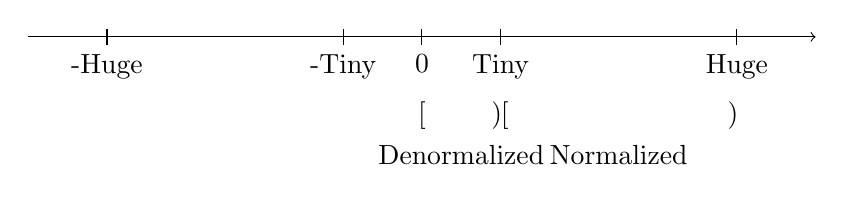
\begin{tikzpicture}
        \draw[->] (-5, 0) -- (5, 0) node[right] {\(\R\)};

        \draw (0, 0.1) -- (0, -0.1) node[below] {0};
        \draw (-4, 0.1) -- (-4, -0.1) node[below] {-Huge};
        \draw (-1, 0.1) -- (-1, -0.1) node[below] {-Tiny};
        \draw (1, 0.1) -- (1, -0.1) node[below] {Tiny};
        \draw (4, 0.1) -- (4, -0.1) node[below] {Huge};

        \node at (0, -1) {[};
        \node at (0.95, -1) {)};
        \node at (1.05, -1) {[};
        \node at (3.95, -1) {)};

        \node at (0.5, -1.5) {Denormalized};
        \node at (2.5, -1.5) {Normalized};
    \end{tikzpicture}
\end{figure}

\begin{table}[H]
    \centering
    \begin{tabular}{ccc}
         & Single
         & Double                                                          \\
        HUGE
         & \( +1.11\dots1 \times 2^{127}   \approx 3.4 \times 10^{38} \)
         & \( +1.11\dots1 \times 2^{1023}  \approx 1.8 \times 10^{308} \)  \\
        TINY
         & \( +1.00\dots0 \times 2^{-126}  \approx 1.2 \times 10^{-38} \)
         & \( +1.00\dots0 \times 2^{-1022} \approx 2.2 \times 10^{-308} \)
    \end{tabular}
\end{table}

\begin{remark}
    What about \( x \in \R \), \( x > \text{HUGE} \)? In this case, we have an overflow, and the computer will return \( fl(x) = +\infty = 1.00\dots0 \times \beta^{u+1} \).
\end{remark}

\begin{remark}
    What happens if we have \( (+ \infty) - (+ \infty) \)? In this case, we have an indeterminate form, and the computer will return \( NaN \) (Not a Number), \[
        1.xx\dots x \times \beta^{u+1}
    \] where at least one of the \( x \)'s is not zero.
\end{remark}

\begin{remark}
    For \( 0 \leq x \leq \text{TINY} \), take \[
        fl(x) = \begin{cases}
            0.00d_id_{i+1}\dots d_{p-1} \times \beta^{L-1} \\
            0 & \text{eventually}
        \end{cases}
    \]
\end{remark}

\begin{example}
    Suppose we have \[
        F(\beta, p, L, U ) = F(10, 3, -10, 10)
    \] and \[
        x = 3.00 \times 10^5, y = 3.00 \times 10^5, \qquad x, y \in \R
    \]

    Computing \[
        z = x^2 + y^2
    \] would give \[
        z = 1.60 \times 10^{11} + 9.00 \times 10^{10} \notin F(10, 3, -10, 10)
    \] and hence \( fl(z) = +\text{Inf} \).

    What if we instead want to compute \[
        z = \sqrt{x^2 + y^2}?
    \]
    Using the standard algorithm, we get +Inf inside the square root, and the computer will return NaN. We need to repair our algorithm.
    \begin{align*}
        h & = \max(|x|, |y|) \times \sqrt{1 + \left(\frac{\min(|x|, |y|)}{\max(|x|, |y|)} \right)^2}
    \end{align*}
\end{example}

\begin{remark}
    The \texttt{libm} library in C and the \texttt{math} module in python both have a function called \texttt{hypot} that computes the Euclidean distance. This is a numerically stable algorithm that avoids overflow and underflow.
\end{remark}

\begin{note}[Inf Could Have Meanings]
    Suppose you are computing the slope of a line, and you get infinity. This would indicate that the line is parallel to the y-axis. This is a meaningful result, and not an error.
\end{note}

\begin{note}[Sometimes, Underflow is OK]
    % Let \( x \in \R \), \( 0 < x < \text{TINY} \).

    % We have \( fl(x) = 0 \), an underflow, but that's OK.

    Recall the McLaurin series for \[
        y = 1 + x + \frac{x^2}{2}
    \]

    Suppose we are computing in \( F(10, 3, -10, 10) \). \[
        y = 1.00 \times 10^0 + 1.00 \times 10^{-5} + 5.00 \times 10^{-11}
    \] The last term would underflow, but that's OK. We can ignore it, since it is negligible.
\end{note}

\section{Computational Errors}

\subsection{Intuition}

\begin{example}
    We know that \( \sqrt{255} = 15.9687194227\dots \), but how should we represent this in our floating point system \( F(\beta, p, L, U) = F(10, 3, -10, 10) \)?

    The easiest solution is \term{chopping} / \term{truncation}, where we only keep the first \( p \) digits. This gives us \[
        fl(\sqrt{255}) = 1.59 \times 10^1
    \]

    Another approach is \term{round to nearest}, which gives us \[
        fl(\sqrt{255}) = 1.60 \times 10^1
    \]
\end{example}

\begin{remark}
    Heath called \( x \in \R \to fl(x) \in F \) \term{rounding}. This is why we use \term{round-to-nearest} to disambiguate.
\end{remark}

\begin{note}
    We can also round to \( +\text{Inf} \) or to \( -\text{Inf} \)
\end{note}

\begin{note}[Banker's Rounding]
    Banker's rounding is a method of rounding that rounds the last digit to the nearest even number, if it is exactly halfway between two numbers. This is the default rounding method in IEEE 754. This method is also known as \term{round to even}.
\end{note}

\begin{example}[Cont.]
    After rounding, we have error \[
        fl(\sqrt{255}) -\sqrt{255} \doteq \begin{cases}
            -0.0687 & \text{chop}             \\
            0.0313  & \text{round-to-nearest}
        \end{cases}
    \]
\end{example}

\begin{definition}[Absolute and Relative Error]
    If \( \tilde{x} \) is an approximation to \( x \), the \term{absolute error in the approximation} is \[
        | \tilde{x} - x |
    \] and the \term{relative error} is \[
        \frac{| \tilde{x} - x |}{|x|} \qquad x \neq 0
    \]
\end{definition}

\begin{example}
    The relative error of the approximation of \( \sqrt{255} \) is \[
        \doteq \begin{cases}
            4.3 \times 10^{-3}  & \text{chop}             \\
            1.96 \times 10^{-3} & \text{round-to-nearest}
        \end{cases}
    \]
\end{example}

\begin{remark}
    Absolute error is not sensitive to scale, while relative error is.
\end{remark}

\begin{example}
    Let \( x, y \in \R \), and they are approximated by \( \tilde{x}, \tilde{y} \in F \).

    Consider \( x = 100.001, y = 0.112, \tilde{x} = 100., \tilde{y} = 0.113 \). The absolute error is \[
        | \tilde{x} - x | = 0.001, \quad | \tilde{y} - y | = 0.001
    \]
    They absolute errors are the same, but this does not meas the two approximations are equally good. The relative error is \[
        \frac{| \tilde{x} - x |}{|x|} \doteq 1.0 \times 10^{-5}, \quad \frac{| \tilde{y} - y |}{|y|} \doteq 9.0
    \] The relative error for \( y \) is much larger than for \( x \), so the approximation for \( y \) is worse.
\end{example}

\subsection{Machine Epsilon}

If \( x \in \R \) is approximated by \( fl(x) \in F \), how large can the relative error be?

\begin{example}
    Consider \( F(10, 3, L, U ), a \in \R \) with \( a = w.xyz \times 10^E \) with \( 0 < w \leq 9 \),  \( 0 \leq x, y, z \leq 9 \), and \( L \leq E \leq U \).

    Assume we determine \( fl(a) \) using round to nearest, \[
        | fl(a) - a | \leq 0.005 \times 10^E
    \]

    The maximum relative error is \begin{align*}
        \max \frac{| fl(a) - a |}{|a|}
         & \leq \frac{\max | fl(a) - a |}{\min | a |}    \\
         & = \frac{0.005 \times 10^E}{1.000 \times 10^E} \\
         & = 0.005 = \frac{1}{2} \times 10^{-2}
    \end{align*}
\end{example}

In general, for \( x \in \R \) and \( fl(x) \in F(\beta, p, L, U) \) with round to nearest, we have \[
    \frac{|fl(x) - x|}{|x|} \leq \frac{1}{2} \times \beta^{1-p}
\] assuming \( x \) is representable.

This quantity is called the \term{relative round-off error bound}.

\begin{definition}[Machine Epsilon]\index{Machine Epsilon}\index{Relative Round-off Error Bound}
    The \term{round-off error bound} or \term{machine epsilon} is the maximum relative error that can occur when approximating a number, \[
        \varepsilon_{\text{machine}} = \frac{1}{2} \times \beta^{1-p}
    \]
\end{definition}

\begin{remark}
    In IEEE 754, we have \[
        \varepsilon_{\text{machine}} = \begin{cases}
            2^{-24} \doteq 5.96 \times 10^{-8} & \text{Single Precision} \\
            2^{-53} \doteq 1.1 \times 10^{-16} & \text{Double Precision}
        \end{cases}
    \]
\end{remark}

\begin{example}
    Suppose we have \( F(10,3, -10, 10) \), \( x = 1.51 \times 10^8 \), and \( y = 3.71 \times 10^6 \) , \( x, y \in \R \), \( fl(x) = x, fl(y) = y \).

    We want to compute \( z = x + y \). We have \[
        z = 1.51 \times 10^8 + 3.71 \times 10^6 = 1.5471 \times 10^8 \notin F.
    \]
\end{example}

\begin{remark}
    Mathematically, addition is not closed in \( F \).
\end{remark}

\begin{note}
    In the CPU, there is extended precision in the floating point unit. This means that the CPU can store more digits than the standard floating point representation. This is useful for intermediate calculations, for example, the \( 0.0371 \times 10^8 \) in the previous example, but the final result is rounded to the standard representation.
\end{note}

\begin{example}[Cont.]
    \[
        fl(z) = \begin{cases}
            1.54 \times 10^8 & \text{chop}             \\
            1.55 \times 10^8 & \text{round-to-nearest}
        \end{cases}
    \]

    We have the relative error \[
        \frac{|fl(x+y) - (x+y)|}{|x+y|} = \begin{cases}
            0.00459 & \text{chop}             \\
            0.00187 & \text{round-to-nearest}
        \end{cases} \leq \varepsilon_{\text{machine}} = \begin{cases}
            0.01  & \text{chop}             \\
            0.005 & \text{round-to-nearest}
        \end{cases}
    \]
\end{example}

\begin{remark}
    For IEEE arithemetic, for \( x, y \in F \) and operation \( \text{op} \in \{ \texttt{+}, \texttt{-,} \texttt{*}, \texttt{/} \} \), we must have \[
        \frac{|fl(x \text{ op } y) -  (x \text{ op } y)|}{|x \text{ op } y|} \leq \varepsilon_{\text{machine}}
    \] and the square root of \( x \) \[
        \frac{|fl(\text{sqrt}(x)) - \sqrt{x}|}{|\sqrt{x}|} \leq \varepsilon_{\text{machine}}
    \]
\end{remark}

How does the error accumulates as we perform more operations?

\begin{example}
    \begin{itemize}
        \item \( \text{expr1} = \text{sqrt}(2.0) + \log(42.0) \)
        \item \( \text{expr1} = \text{exp}(7.0) + \sin(45.0) \)
    \end{itemize}

    We have \[
        \varepsilon_{\text{expr1}} = \frac{|\text{expr1} - (\sqrt{2} + \ln(42))|}{|\sqrt{2} + \ln(42)|}
    \] and \[
        \varepsilon_{\text{expr2}} = \frac{|\text{expr2} - (e^7 + \sin(45))|}{|e^7 + \sin(45)|}
    \]

    Suppose we compute \[
        \text{expr1} + \text{expr2} \qquad \text{expr1} \times \text{expr2} \qquad \text{expr1} \div \text{expr2}
    \]

    We know that
    \begin{itemize}
        \item \( \varepsilon_{\text{expr1} + \text{expr2}} \leq \max( \varepsilon_{\text{expr1}}, \varepsilon_{\text{expr2}}) + | \epsilon_A | \)
        \item \( \varepsilon_{\text{expr1} \times \text{expr2}} \leq \varepsilon_{\text{expr1}} + \varepsilon_{\text{expr2}} + | \epsilon_B | \)
        \item \( \varepsilon_{\text{expr1} \div \text{expr2}} \leq \varepsilon_{\text{expr1}} + \varepsilon_{\text{expr2}} + | \epsilon_C | \)
    \end{itemize}

    The first terms are error due to in exact operands. The last terms are due to the representing the result in floating point, and since they are representation errors, they need to be smaller than the machine epsilon, \[
        | \epsilon_A |, | \epsilon_B |, | \epsilon_C | \leq \varepsilon_{\text{machine}}
    \]
\end{example}

\begin{remark}
    Error does not grow too quickly, but it does grow. This is why we need to be careful when performing many operations.
\end{remark}

What about subtraction? That is a whole different story.

\subsection{Catastrophic Cancellation}

\begin{example}
    Suppose we want to find the roots of \[
        x^2 + (-320x) + 16 = 0.
    \] From math textbooks, we know the quadratic formula \[
        r_{1,2} = \frac{-b \pm \sqrt{b^2 - 4ac}}{2a}
    \]

    Using \( F(10, 4, L, U) \), we have \begin{align*}
        r_1 & = \frac{3.200 \times 10^2 + \sqrt{1.024 \times 10^5 - 6.400 \times 10^1}}{2.000 \times 10^0} \\
            & \doteq \frac{3.200 \times 10^2 + \sqrt{1.023 \times 10^5}}{2.000 \times 10^0}
            & \text{1 round off error}                                                                     \\
            & \doteq \frac{3.200 \times 10^2 + 3.198 \times 10^2}{2.000 \times 10^0}                       \\
            & = \frac{6.398 \times 10^2}{2.000 \times 10^0}                                                \\
            & = 3.199 \times 10^2
    \end{align*}

    Similarly,
    \begin{align*}
        r_2 & = \frac{3.200 \times 10^2 - \sqrt{1.024 \times 10^5 - 6.400 \times 10^1}}{2.000 \times 10^0} \\
            & \doteq \frac{3.200 \times 10^2 - \sqrt{1.023 \times 10^5}}{2.000 \times 10^0}
            & \text{1 round off error}                                                                     \\
            & \doteq \frac{3.200 \times 10^2 - 3.198 \times 10^2}{2.000 \times 10^0}                       \\
            & = \frac{2.000 \times 10^{-1}}{2.000 \times 10^0}                                             \\
            & = 1.000 \times 10^{-1}
    \end{align*}

    You can show that the exact roots are \[
        r_1^* \doteq 319.950 \quad r_2^* \doteq 0.050 \qquad r_2^* = 0.05001
    \]

    So the relative errors \[
        \varepsilon_{r_1} \doteq 1.6 \times 10^{-4} \leq \varepsilon_{\text{machine}} = 5 \times 10^{-4} \qquad \varepsilon_{r_2} \doteq 1.0
    \]
\end{example}

\begin{remark}
    A machine epsilon of \( 1 \) tells us that the result is completely wrong. There is no digits of accuracy in the result.
\end{remark}

Why would this happen? \[
    r_2 = \frac{3.200 \times 10^2 - 3.198 \times 10^2}{2.000 \times 10^0}
\]

We know that
\begin{itemize}
    \item \( 3.200 \times 10^2 \) is exact
    \item \( 3.198 \times 10^2 \) has 2 rounding errors, \( fl(\sqrt{fl(102400 - 64)}) \)
    \item \( 2.000 \times 10^0 \) is exact
\end{itemize}

We wanted to subtract \[
    3.200 \times 10^2 - 3.198\texttt{xxxxxx} \times 10^2
\] We see that the leading terms cancel out, and \( \texttt{xxxxxx} \) are insignificant in the intermediate result, but they are significant in the final result. This is know as the \term{catastrophic cancellation}.

\begin{definition}[Catastrophic Cancellation]\index{Catastrophic Cancellation}
    \term{Catastrophic Cancellation} is the loss of significance in the result in subtracting two possibly inexact quantities close in value.
\end{definition}

\begin{remark}
    To avoid catastrophic cancellation, avoid subtracting nearly equal inexact quantities.
\end{remark}

\begin{example}[Cont.]
    So how to determine \( r_2 \) accurately?

    We know that \[
        ( 1x^2 - 320x + 16 ) = 1 \cdot ( x - r_1 ) ( x - r_2 )
    \] so
    \begin{itemize}
        \item \( 1 \cdot r_1 r_2 = 16 \) when \( x = 0 \)
        \item \( r_2 = \dfrac{16}{r_1} = \frac{1.600 \times 10^1}{3,199 \times 10^2} = 5.002 \times 10^{-2} < \epsilon_{\text{machine}} \)
    \end{itemize}
\end{example}

\begin{remark}
    A better algorithm to compute roots of \[
        ax^2 + bx + c = 0
    \] is \[
        r_1 = \frac{-b - \text{sign}(b) \sqrt{b^2 - 4ac}}{2a} \qquad r_2 = \frac{c}{ar_1}
    \]
\end{remark}

Why there is no catastrophic cancellation in \( b^2 - 4ac \)?

If there is cancellation, we must have \( b^2 \approx 4ac \), which means their difference would be a small number, and the square root would be a small number. We later adds it with a much bigger number \( b \), so the small number is insignificant, and the inaccuracy here does not affect the final result.

\begin{example}
    Consider \( F(10, 4, L, U) \), \( x = 1,23 \times 10^1 \), and \( y = 2.3xx \times 10^{-2} \).

    We have \begin{align*}
        x + y
         & = 12.34 + 0.023\texttt{xx}                                                 \\
         & = 12.363\texttt{xx} \xrightarrow{\text{round}} fl(x+y) = 1.236 \times 10^1
    \end{align*}
\end{example}

\begin{remark}
    Given expr1 and expr2, with all positive intermediate results, \[
        \varepsilon_{\text{expr1} - \text{expr2}} \leq \left| \frac{\text{expr1}}{\text{expr1}-\text{expr2}} \right| \varepsilon_{\text{expr1}} + \left| \frac{\text{expr2}}{\text{expr1}-\text{expr2}} \right| \varepsilon_{\text{expr2}} + \varepsilon_{D}
    \] where \( \varepsilon_{D} < \varepsilon_{\text{machine}} \) is the representation error.
\end{remark}

\begin{remark}
    Software try to avoid the subtraction of 2 nearly equal inexact values.
\end{remark}

\begin{example}
    Give an accurate algorithm for computing the value of \[
        f(x) = \sqrt{1 + x} - 1
    \] for \( x > 0 \).

    The na\"ive approach would be to compute \[
        \texttt{f = math.sqrt(1 + x) - 1}
    \] but this would lead to catastrophic cancellation when \( x \) is small. The significant of any error in \texttt{math.sqrt(1+x)} is revealed by the subtraction.

    A work around is to compute \begin{align*}
        f(x)
         & = (\sqrt{1+x} - 1) \cdot \frac{\sqrt{1+x}+1}{\sqrt{1+x}+1} \\
         & = \frac{(1+x) - 1}{\sqrt{1+x} + 1}                         \\
         & = \frac{x}{\sqrt{1+x} + 1}
    \end{align*} and since \( x > 0 \), there is no catastrophic cancellation. A trade off, however, is that this approach is slower than the na\"ive approach as we have 1 more operation.


    \begin{algorithmic}
        \Function{f}{$x$}
        \If{\( x \geq 3 \)}
        \State \( f = \texttt{math.sqrt(1+x) - 1} \)
        \Else
        \State \( f = \texttt{x / (math.sqrt(1+x) + 1)} \)
        \EndIf
        \EndFunction
    \end{algorithmic}
\end{example}

\begin{definition}[Numerically Stable Algorithm]\index{Numerically Stable Algorithm}
    An algorithm is said to be \term{numerically stable} if the result it produces is the exact result of a ``nearby'' problem.
\end{definition}

\begin{example}
    \setlength{\parindent}{0pt}

    Recall computing the root for \[
        1 \cdot x^2 + (-320)x + 16 = 0
    \]

    Recall also \[
        ax^2 + bx + c = 0 \qquad a(x - r_1)(x - r_2) = 0
    \] are two ways to express the quadratic.

    The quadratic formula gives \[
        r_1 \ 3.199 \times 19^2 \quad r_2 = 1.000 \times 10^{-1}
    \]

    For which quadratic equation is this the exact solution? \[
        1(x - 3.199 \times 10^2)(x - 1.000 \times 10^{-1}) = 0
    \] which is the same as \[
        x^2 - 320x + 31.99 = 0
    \]

    We got the exact roots of a very different problem, \( 16 \to 31.99 \) with a relative increment \( \approx 1 \).

    {~~~}

    The later modifier algorithm gave us \[
        r_1 = 3.199 \times 10^2 \quad r_2 = 5.002 \times 10^{-2}
    \]

    Fir which quadratic equation is this the exact solution? \[
        1(x - 3.199 \times 10^2)(x - 5.002 \times 10^{-2}) = 0
    \] which is the same as \[
        x^2 - 319.95002x + 16.001398 = 0
    \]

    The difference 
    \begin{itemize}
        \item \( \Delta a = 0 \)
        \item \( \Delta b = 0.04998 \) with relative change \( \doteq 1.56 \times 16^4 < \varepsilon_{\text{machine}} \)
        \item \( \Delta c = 0.01398 \) with relative change \( \doteq 8.74 \times 10^{-5} < \varepsilon_{\text{machine}} \)
    \end{itemize}
\end{example}